

\begin{frame}{Benchmark}
  \begin{center} \Large \textbf{Histograms} \end{center}
\end{frame}

\begin{frame}{Benchmark}
  \begin{center} 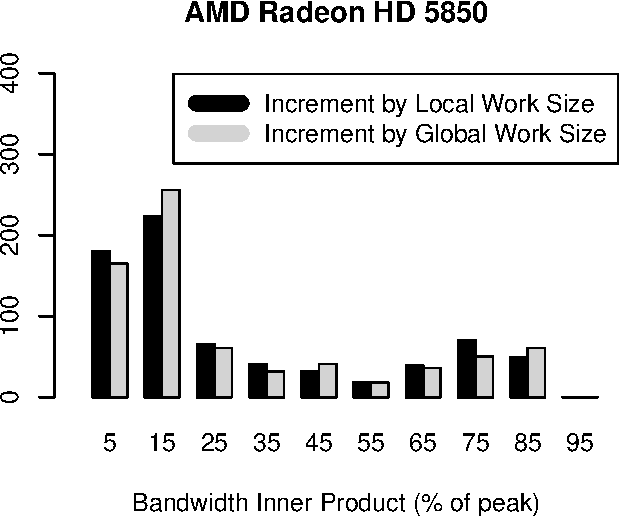
\includegraphics[width=0.75\textwidth]{figures/hd5850_double_hist_itertype_dot} \end{center}
\end{frame}

\begin{frame}{Benchmark}
  \begin{center} 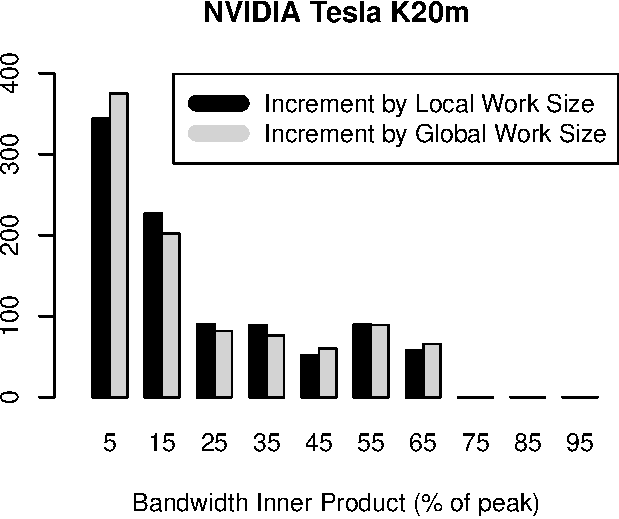
\includegraphics[width=0.75\textwidth]{figures/k20m_double_hist_itertype_dot} \end{center}
\end{frame}

\begin{frame}{Benchmark}
  \begin{center} 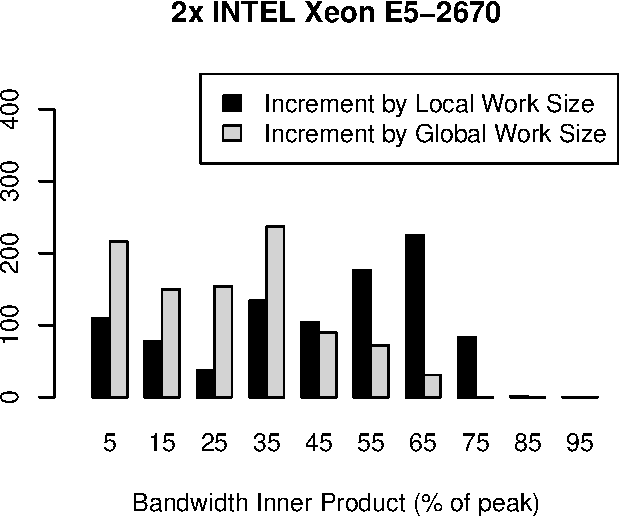
\includegraphics[width=0.75\textwidth]{figures/xeon_cpu_double_hist_itertype_dot} \end{center}
\end{frame}

\begin{frame}{Benchmark}
  \begin{center} 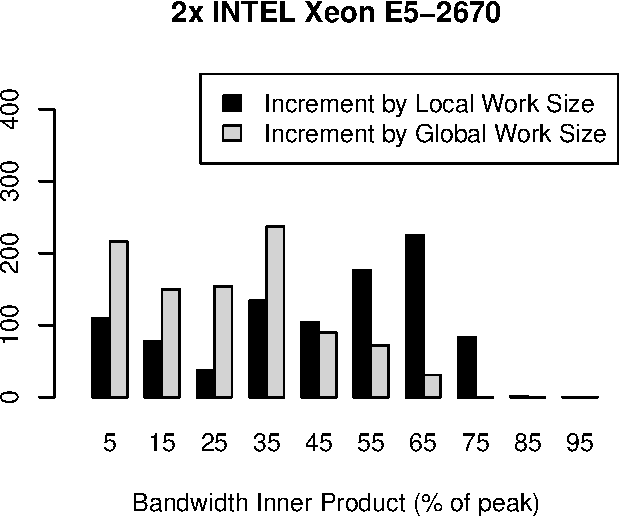
\includegraphics[width=0.55\textwidth]{figures/xeon_cpu_double_hist_itertype_dot} \\[1em]
                 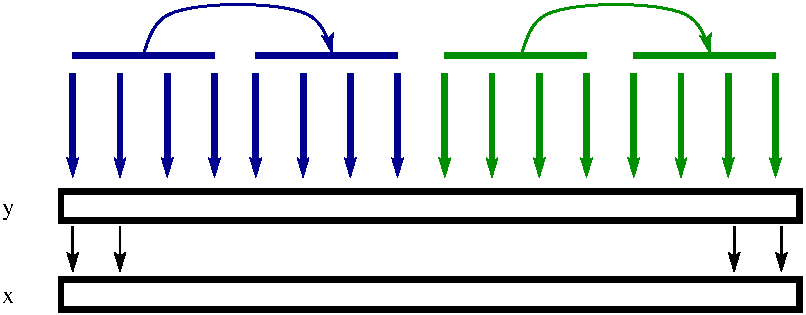
\includegraphics[width=0.45\textwidth]{figures/copy-kernel-cpu-full} 
  \end{center}
\end{frame}

\begin{frame}{Benchmark}
  \begin{center} 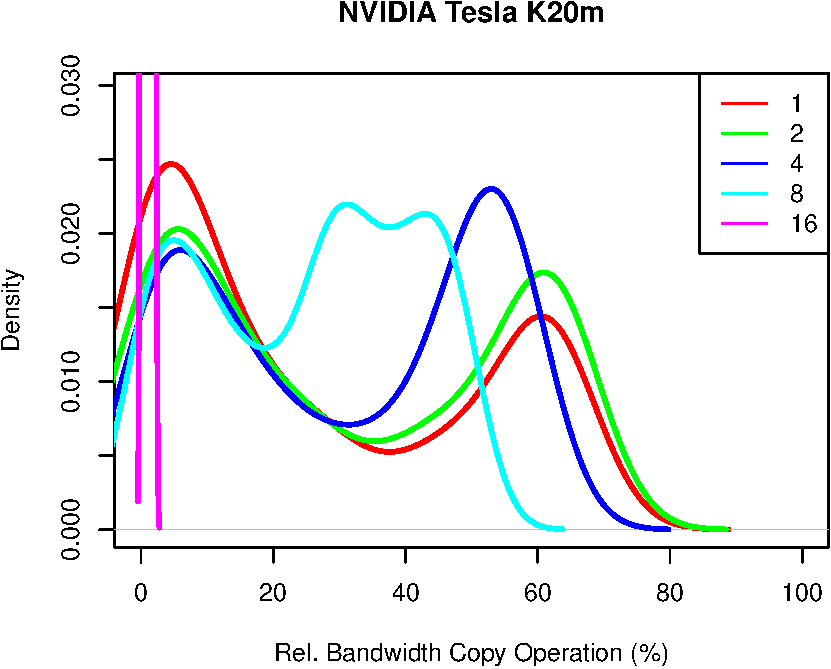
\includegraphics[width=0.75\textwidth]{figures/k20m_double_hist_vec_copy-crop} \\
                  \footnotesize (comparison of vector types \texttt{double, double2, double4, double8, double16}) \end{center}
\end{frame}

\begin{frame}{Benchmark}
  \begin{center} 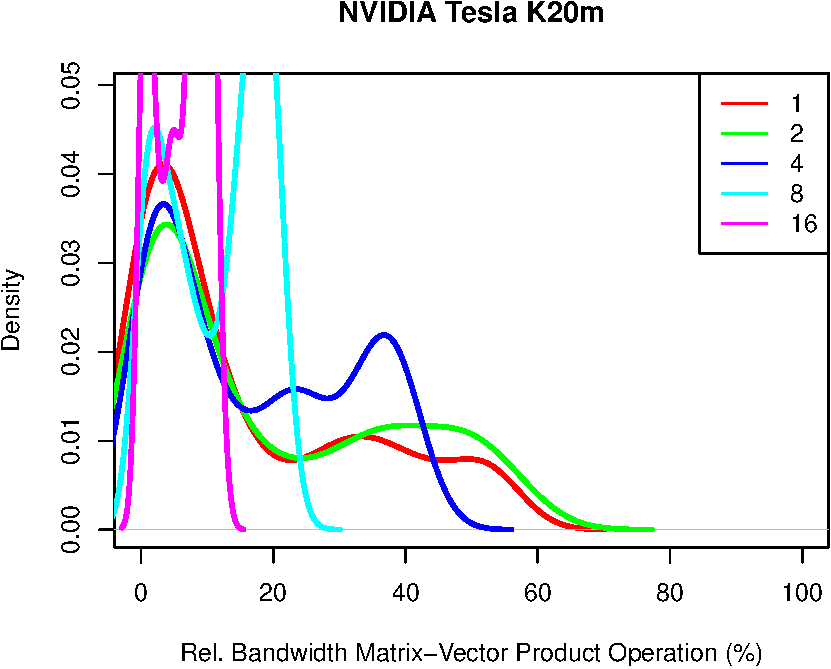
\includegraphics[width=0.75\textwidth]{figures/k20m_double_hist_vec_gemv-crop} \\
                  \footnotesize (comparison of vector types \texttt{double, double2, double4, double8, double16})  \end{center}
\end{frame}



%%%%%%%%%%%%%%%%%%%%%%%%%%%%%%%%%%%%%%%%%%%%%%%%%%%%%%%%%%%%%%%


\begin{frame}{Benchmark}
  \begin{center} \textbf{ [Addition$|$Inner Product$|$Matrix-Vector] vs. Copy Kernel }\\[1em] Same Device \end{center}
\end{frame}

\begin{frame}{Benchmark}
  \only<1>{\begin{center} 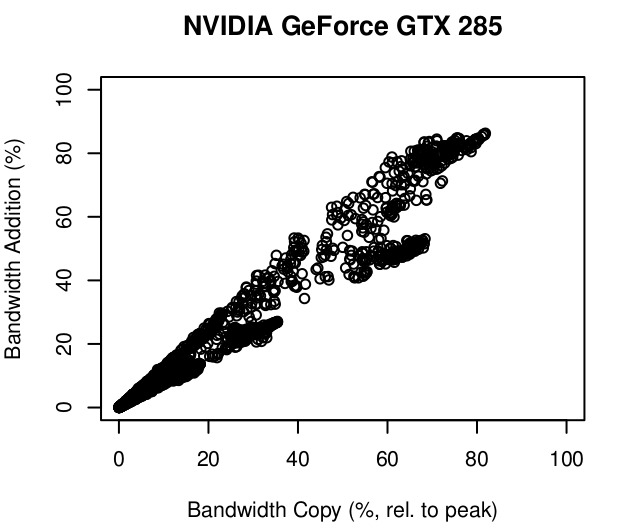
\includegraphics[width=0.8\textwidth]{figures/gtx285-addition-copy-1} \end{center}}
  \only<2>{\begin{center} 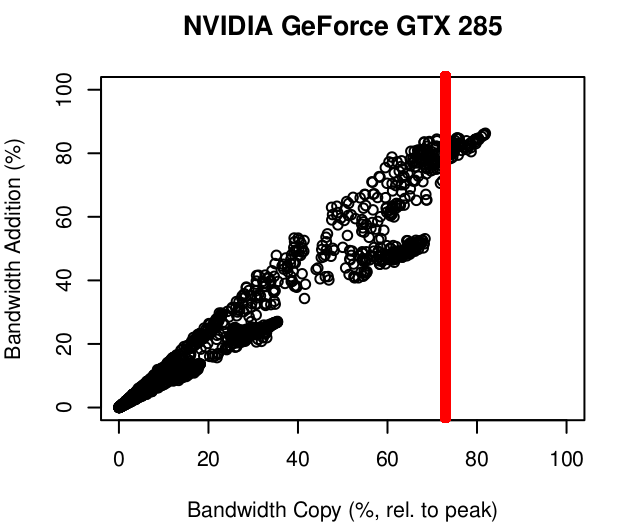
\includegraphics[width=0.8\textwidth]{figures/gtx285-addition-copy-2} \end{center}}
  \only<3>{\begin{center} 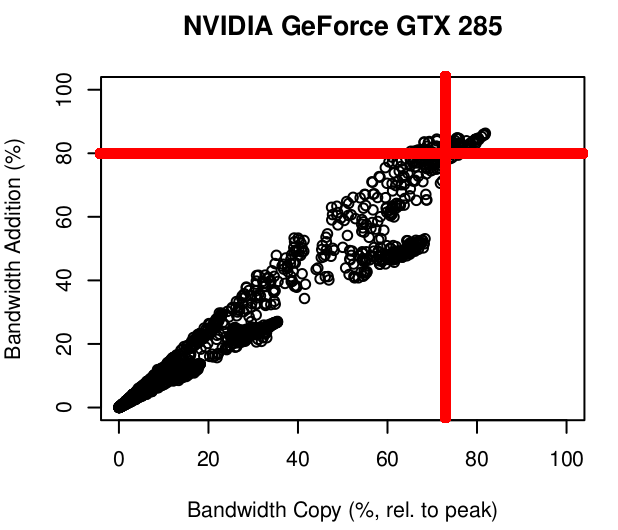
\includegraphics[width=0.8\textwidth]{figures/gtx285-addition-copy-3} \end{center}}
\end{frame}


\begin{frame}{Benchmark}
  \begin{center} \end{center}
  \only<1>{\begin{center} {\LARGE NVIDIA Tesla K20m} \\[2em]       \hspace*{1.cm} Addition \hspace*{2.1cm} Inner Product \hspace*{1.4cm} Mat-Vec Product \\[1em] 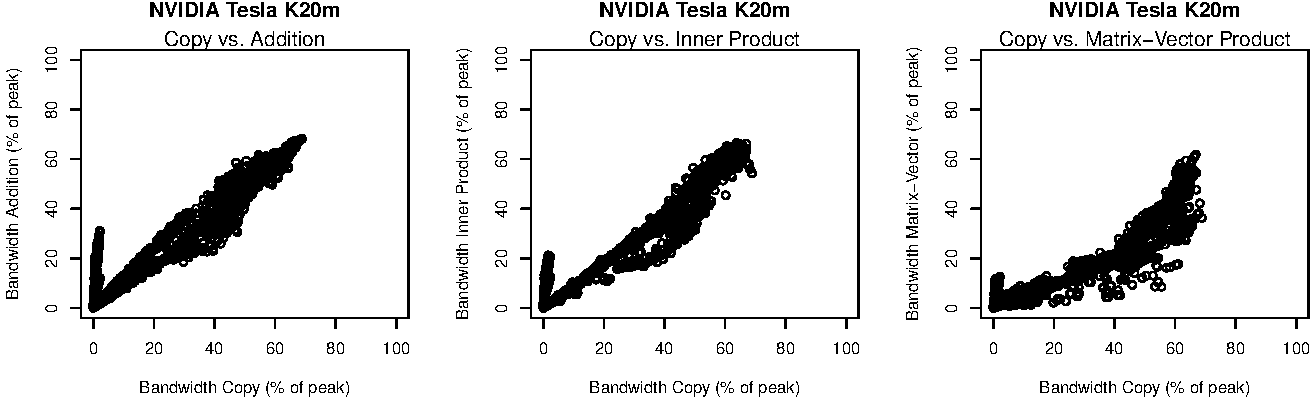
\includegraphics[width=0.99\textwidth]{figures/k20m_double_xy_copy-crop} \end{center}}
  \only<2>{\begin{center} {\LARGE AMD Radeon HD 5850} \\[2em]      \hspace*{1.cm} Addition \hspace*{2.1cm} Inner Product \hspace*{1.4cm} Mat-Vec Product \\[1em] 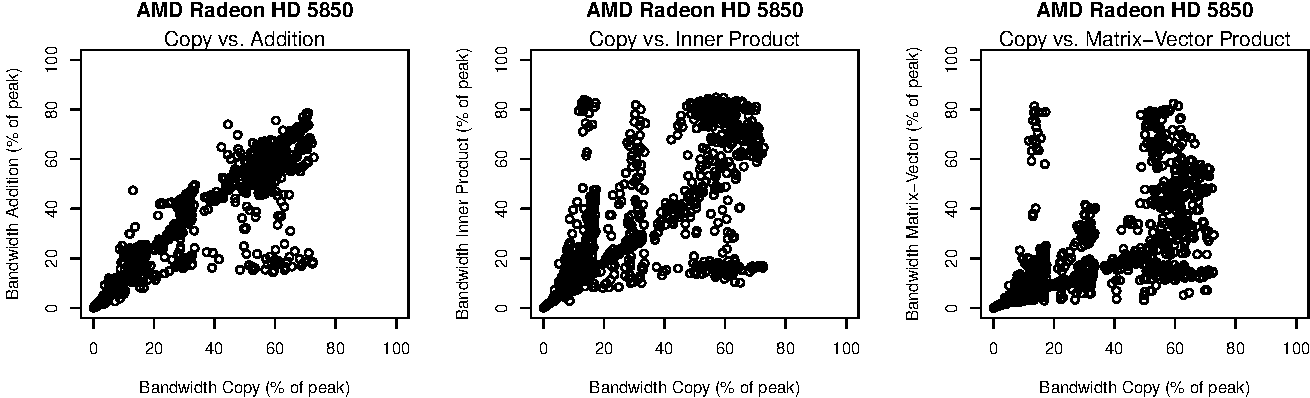
\includegraphics[width=0.99\textwidth]{figures/hd5850_double_xy_copy-crop} \end{center}}
  \only<3>{\begin{center} {\LARGE INTEL Dual Xeon E5-2670} \\[2em] \hspace*{1.cm} Addition \hspace*{2.1cm} Inner Product \hspace*{1.4cm} Mat-Vec Product \\[1em] 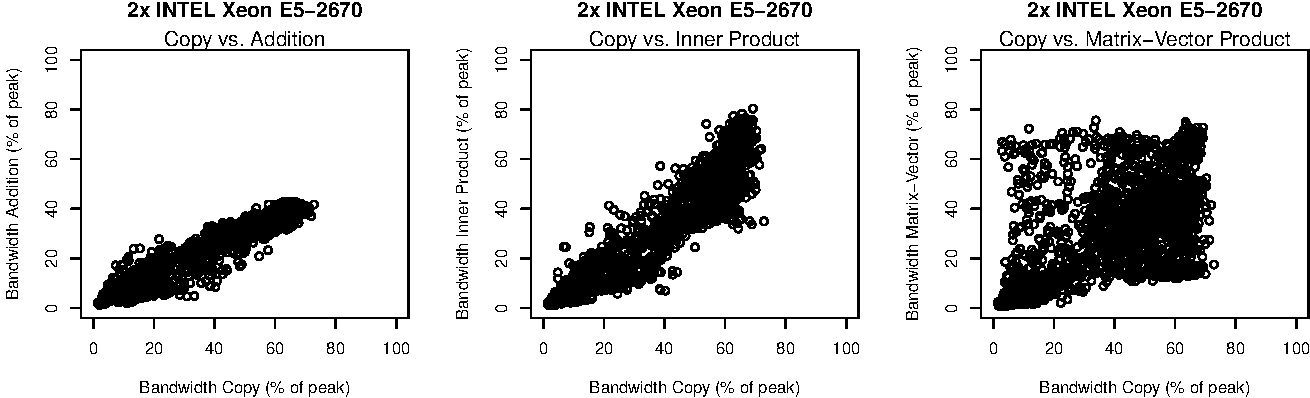
\includegraphics[width=0.99\textwidth]{figures/xeon_cpu_double_xy_copy-crop} \end{center}}
  \only<4>{\begin{center} {\LARGE INTEL Xeon Phi} \\[2em]          \hspace*{1.cm} Addition \hspace*{2.1cm} Inner Product \hspace*{1.4cm} Mat-Vec Product \\[1em] 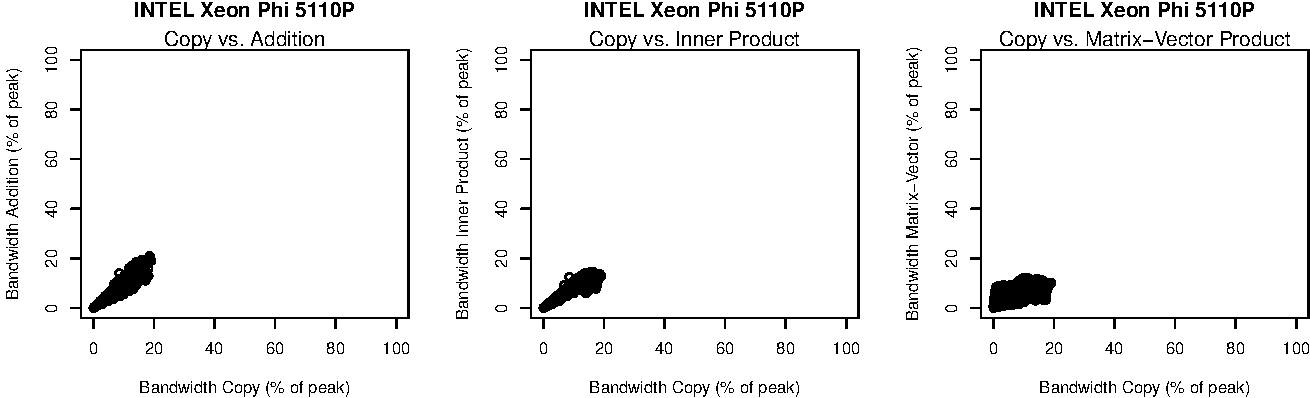
\includegraphics[width=0.99\textwidth]{figures/xeon_phi_float_xy_copy-crop} \end{center}}
\end{frame}

\begin{frame}{Benchmark}
  \begin{center} Conclusio: \\[1em] {\Large Focus on fastest configurations for copy-kernel sufficient}  \end{center}
\end{frame}



%%%%%%%%%%%%%%%%%%%%%%%%%%%%%%%%%%%%%%%%%%%%%%%%%%%%%%%%%%%%%%%


\begin{frame}{Benchmark}
  \begin{center} \textbf{ [Copy$|$Addition$|$Inner Product$|$Matrix-Vector] vs. Copy Kernel }\\[1em] Different Device, Same Vendor \end{center}
\end{frame}

\begin{frame}{Benchmark}
  \only<1>{\begin{center} \LARGE \hspace*{1.5cm} NVIDIA Hardware (x: GTX 285, y: K20m) \\[1em] 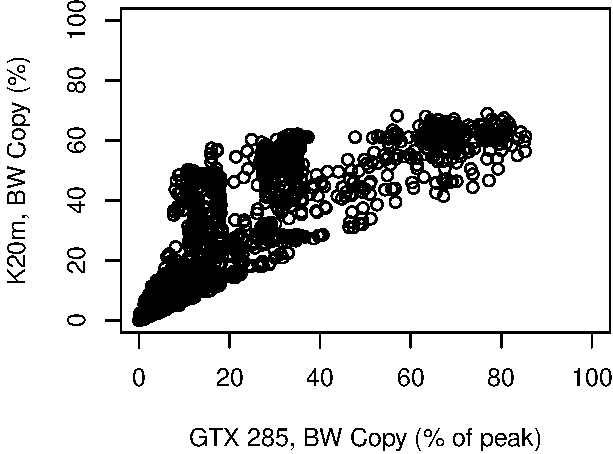
\includegraphics[width=0.75\textwidth]{figures/gtx_285_double_k20m_double_copy-crop} \end{center}}
  \only<2>{\begin{center} \LARGE \hspace*{1.7cm} AMD Hardware (x: A10-5800K GPU, y: HD 5850)  \\[1em]    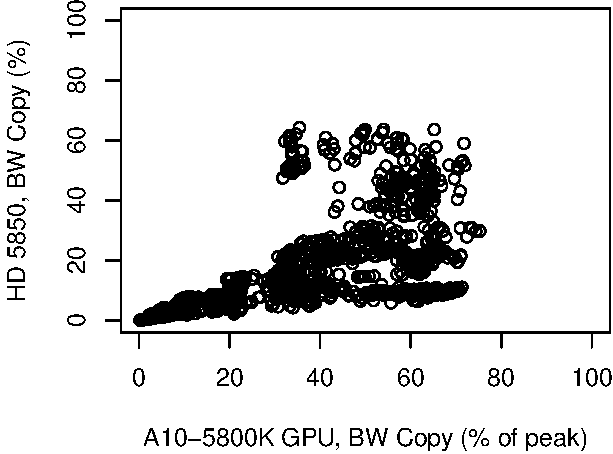
\includegraphics[width=0.75\textwidth]{figures/a10_5800K_devastator_float_hd5850_float_copy-crop} \end{center}}
  \only<3>{\begin{center} \LARGE \hspace*{1.7cm} INTEL Hardware (x: Xeon Phi, E5-2670) \\[1em]  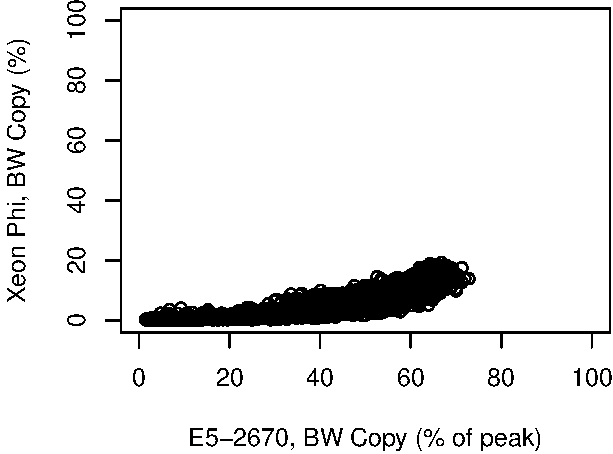
\includegraphics[width=0.75\textwidth]{figures/xeon_cpu_double_xeon_phi_float_copy-crop} \end{center}}
\end{frame}

\begin{frame}{Benchmark}
  \only<1>{\begin{center} {\LARGE NVIDIA Hardware (x: GTX 285, y: K20m) } \\[1em]         \hspace*{1.cm} Addition \hspace*{2.1cm} Inner Product \hspace*{1.4cm} Mat-Vec Product \\[1em]  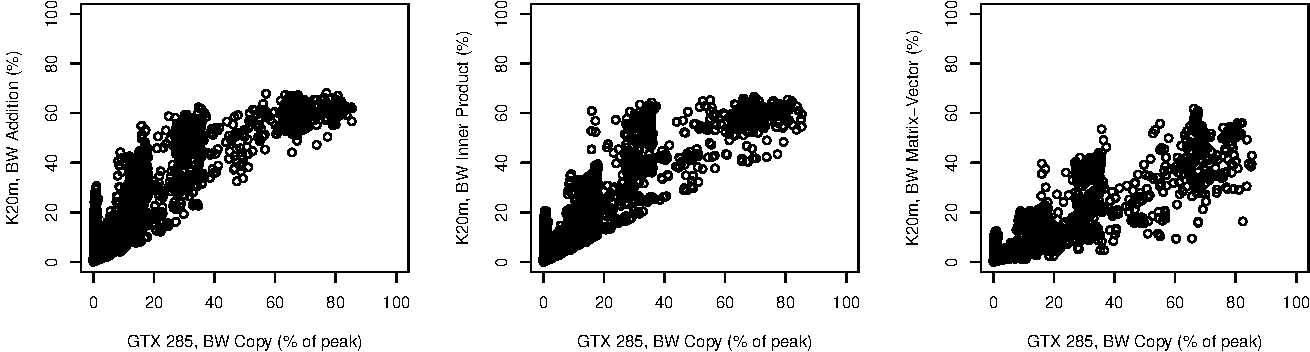
\includegraphics[width=0.99\textwidth]{figures/gtx_285_double_k20m_double_kernels-crop} \end{center}}
  \only<2>{\begin{center} {\LARGE AMD Hardware (x: A10-5800K GPU, y: HD 5850) } \\[1em]   \hspace*{1.cm} Addition \hspace*{2.1cm} Inner Product \hspace*{1.4cm} Mat-Vec Product \\[1em]  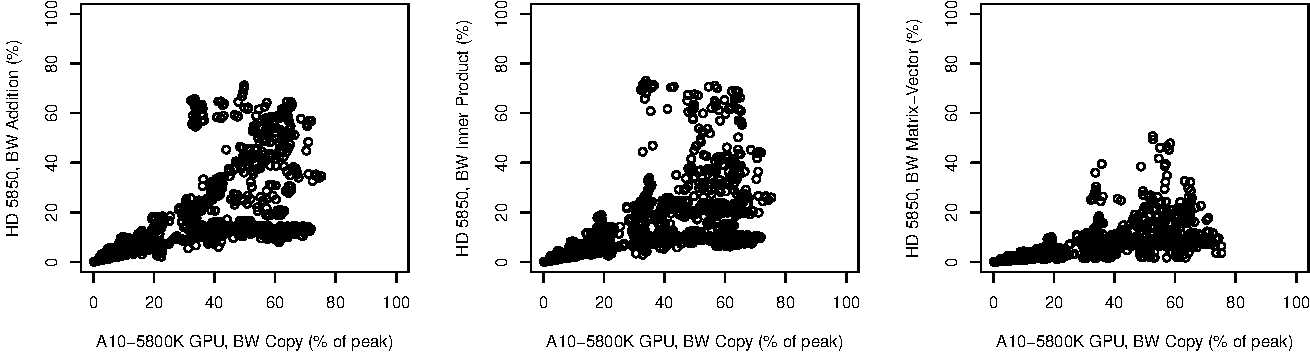
\includegraphics[width=0.99\textwidth]{figures/a10_5800K_devastator_float_hd5850_float_kernels-crop} \end{center}}
\end{frame}

\begin{frame}{Benchmark}
  \begin{center} Conclusio: \\[1em] {\Large Certain Performance Portability per Vendor}  \end{center}
\end{frame}


%%%%%%%%%%%%%%%%%%%%%%%%%%%%%%%%%%%%%%%%%%%%%%%%%%%%%%%%%%%%%%%


\begin{frame}{Benchmark}
  \begin{center} \textbf{ [Copy$|$Addition$|$Inner Product$|$Matrix-Vector] vs. Copy Kernel }\\[1em] Different Device, Different Vendor \end{center}
\end{frame}

\begin{frame}{Benchmark}
  \only<1>{\begin{center} \LARGE \hspace*{1.7cm} x: INTEL CPU, y: AMD CPU \\[0.5em]    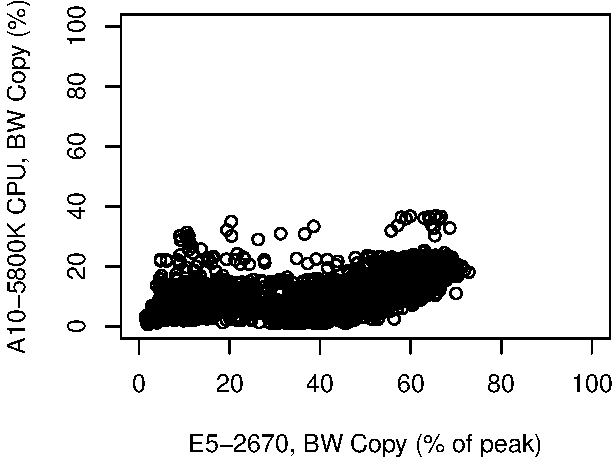
\includegraphics[width=0.75\textwidth]{figures/xeon_cpu_double_a10_5800K_cpu_double_copy-crop} \end{center}}
  \only<2>{\begin{center} \LARGE \hspace*{1.5cm} x: INTEL CPU, y: NVIDIA GPU \\[0.5em] 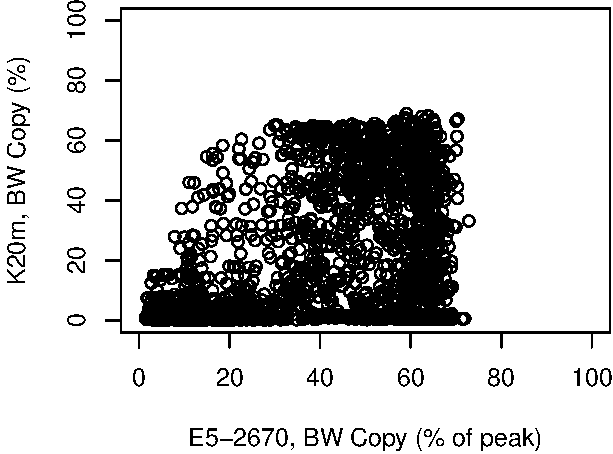
\includegraphics[width=0.75\textwidth]{figures/xeon_cpu_double_k20m_double_copy-crop} \end{center}}
  \only<3>{\begin{center} \LARGE \hspace*{1.7cm} x: AMD GPU, y: NVIDIA GPU \\[0.5em]   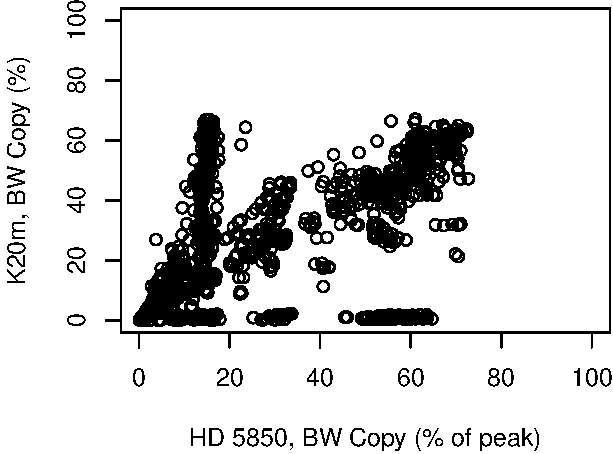
\includegraphics[width=0.75\textwidth]{figures/hd5850_double_k20m_double_copy-crop} \end{center}}
\end{frame}


\begin{frame}{Benchmark}
  \only<1>{\begin{center} {\LARGE x: AMD HD 5850, y: NVIDIA K20m} \\[2em] \hspace*{1.cm} Addition \hspace*{2.1cm} Inner Product \hspace*{1.4cm} Mat-Vec Product \\[1em] 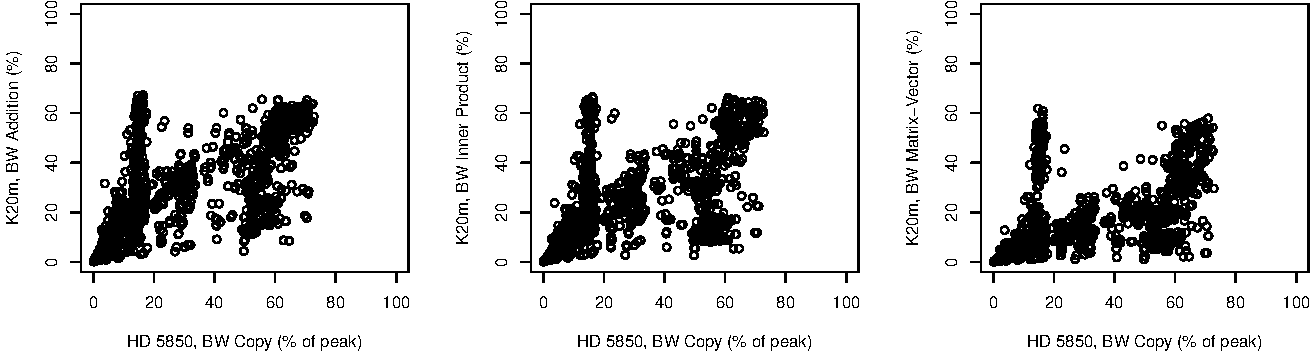
\includegraphics[width=0.99\textwidth]{figures/hd5850_double_k20m_double_kernels-crop} \end{center}}
\end{frame}

\begin{frame}{Benchmark}
  \begin{center} Conclusio: \\[1em] {\Large Fast Configurations Across Vendors Exist}  \end{center}
\end{frame}


%%%%%%%%%%%%%%%%%%%%%%%%%%%%%%%%%%%%%%%%%%%%%%%%%%%%%%%%%%%%%%%

% 
% \begin{frame}{Benchmark}
%   \begin{center} \textbf{ \LARGE Matrix-Matrix Multiplication }  \\[1em] Single Precision \end{center}
% \end{frame}
% 
% 
% \begin{frame}{Benchmark}
%   \only<1>{\begin{center} 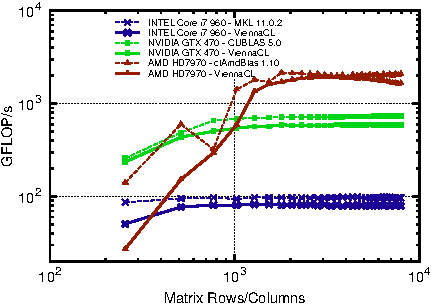
\includegraphics[width=0.8\textwidth]{figures/sgemm}  \end{center} {\small Ph.~Tillet \textit{et al.}: HotPar'13}}
%   \only<2>{\begin{center} \includegraphics[width=0.85\textwidth]{figures/gtx_470_float_xy} \end{center}}
% \end{frame}
% 
